\begin{figure}[t]
	\centering
	\subfloat[学到的 Frey Face 流形]{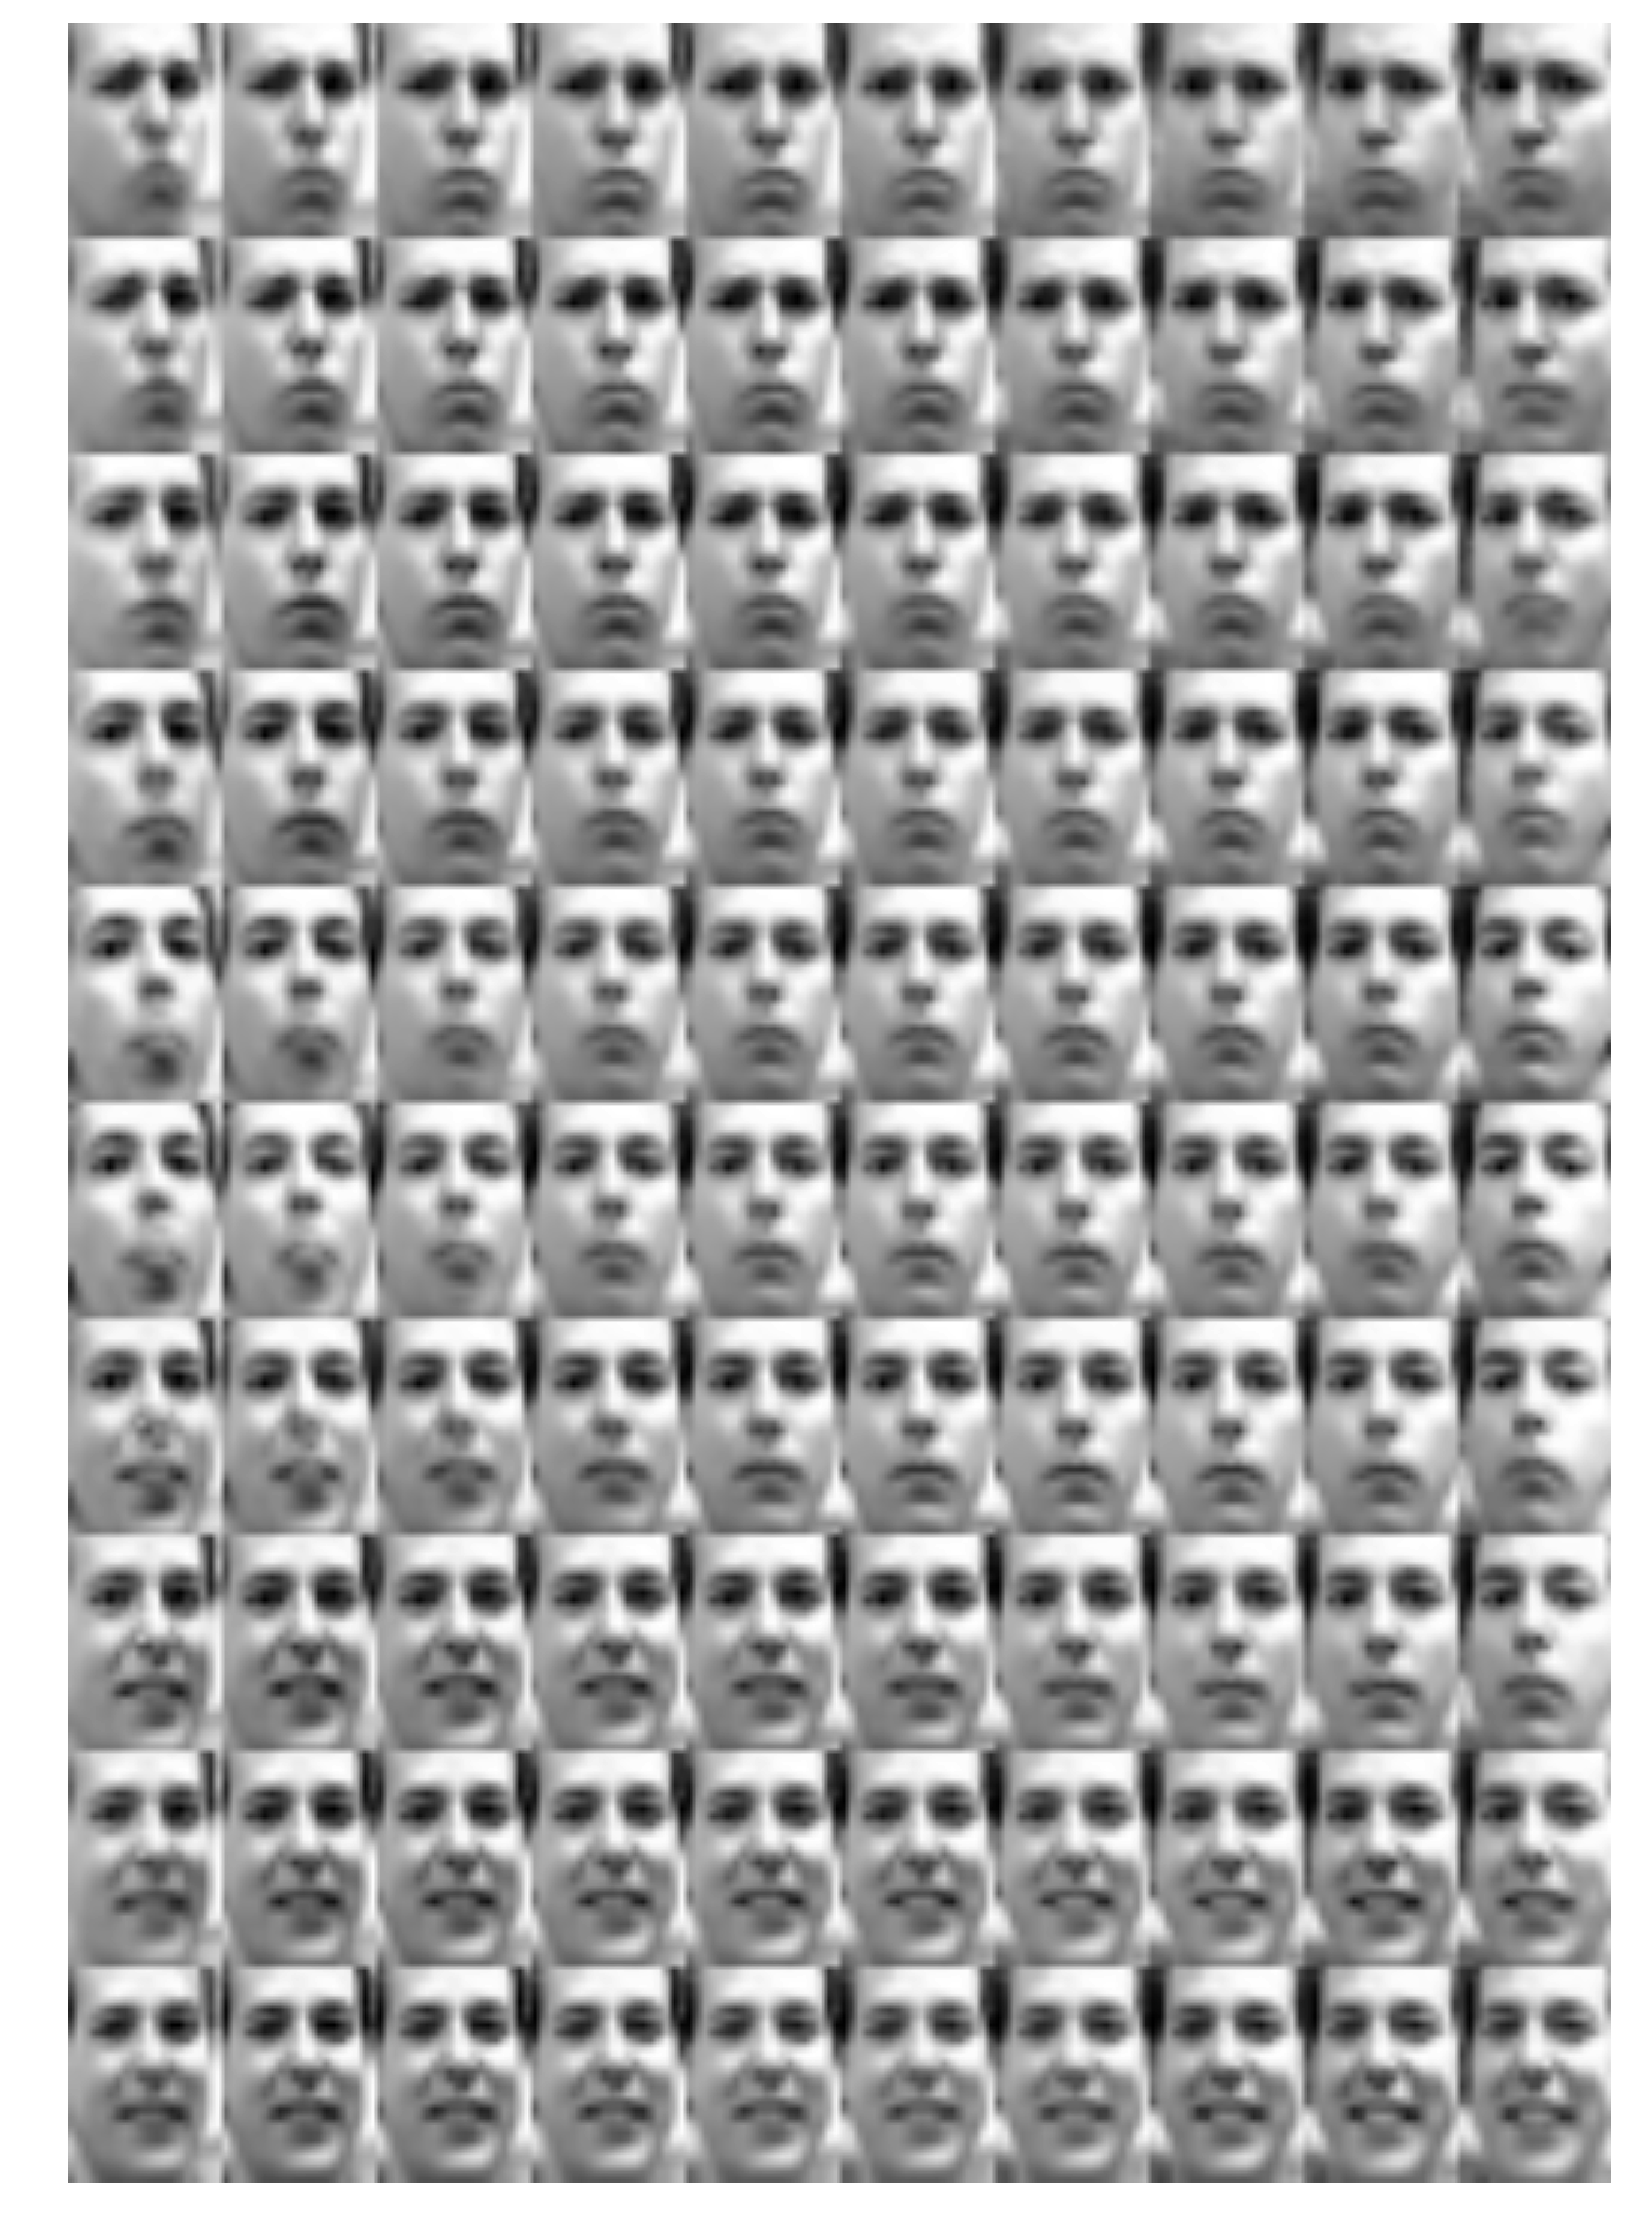
\includegraphics[width=0.33\textwidth]{assets/figures/freyface_10x10.pdf}}
        ~ 
	\subfloat[学到的 MNIST 流形]{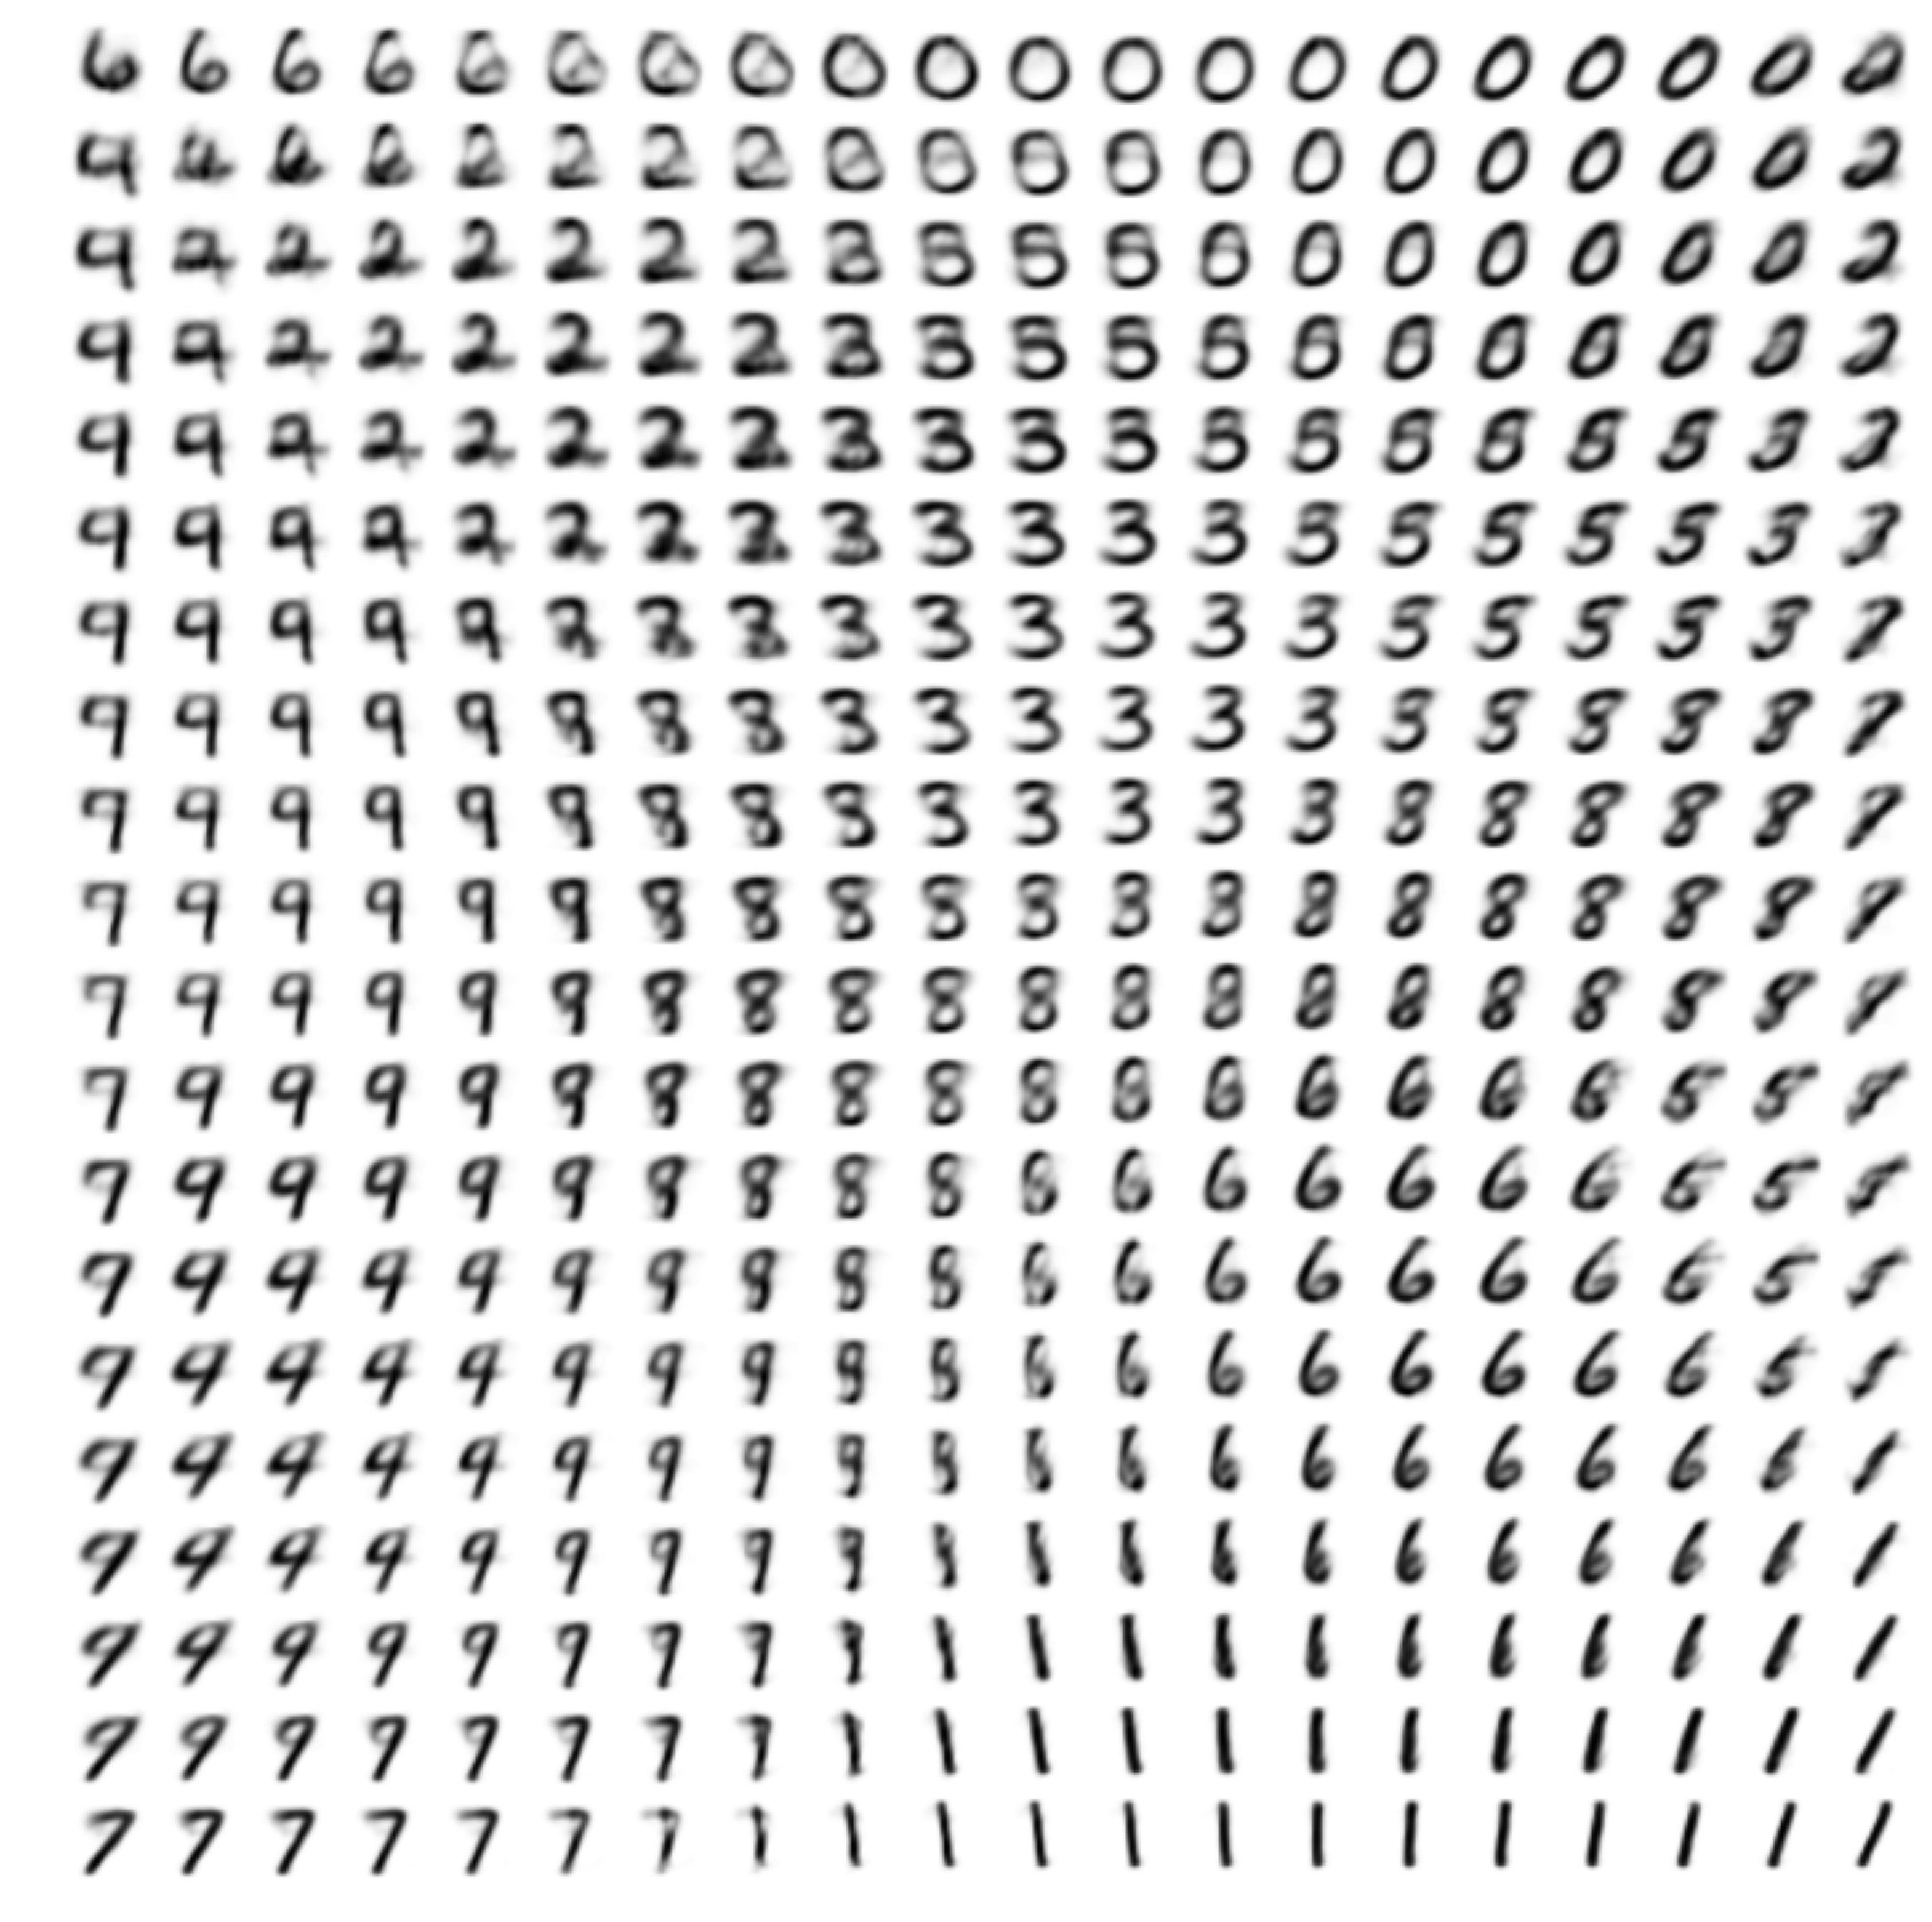
\includegraphics[width=0.57\textwidth]{assets/figures/mnist_20x20.pdf}}
\caption{通过 AEVB 学到的二维潜在空间生成模型的数据流形可视化。由于潜在空间的先验为高斯分布，将单位正方形内线性等距的坐标通过高斯分布的逆 CDF 变换，得到潜变量 $\bz$ 的取值。对每个 $\bz$，利用学到的参数 $\bT$，绘制相应生成分布 $\pT(\bx|\bz)$ 的图像。}
\label{fig:2dmanifolds}
\end{figure}

\begin{figure}[h]
	\centering
	\subfloat[二维潜在空间]{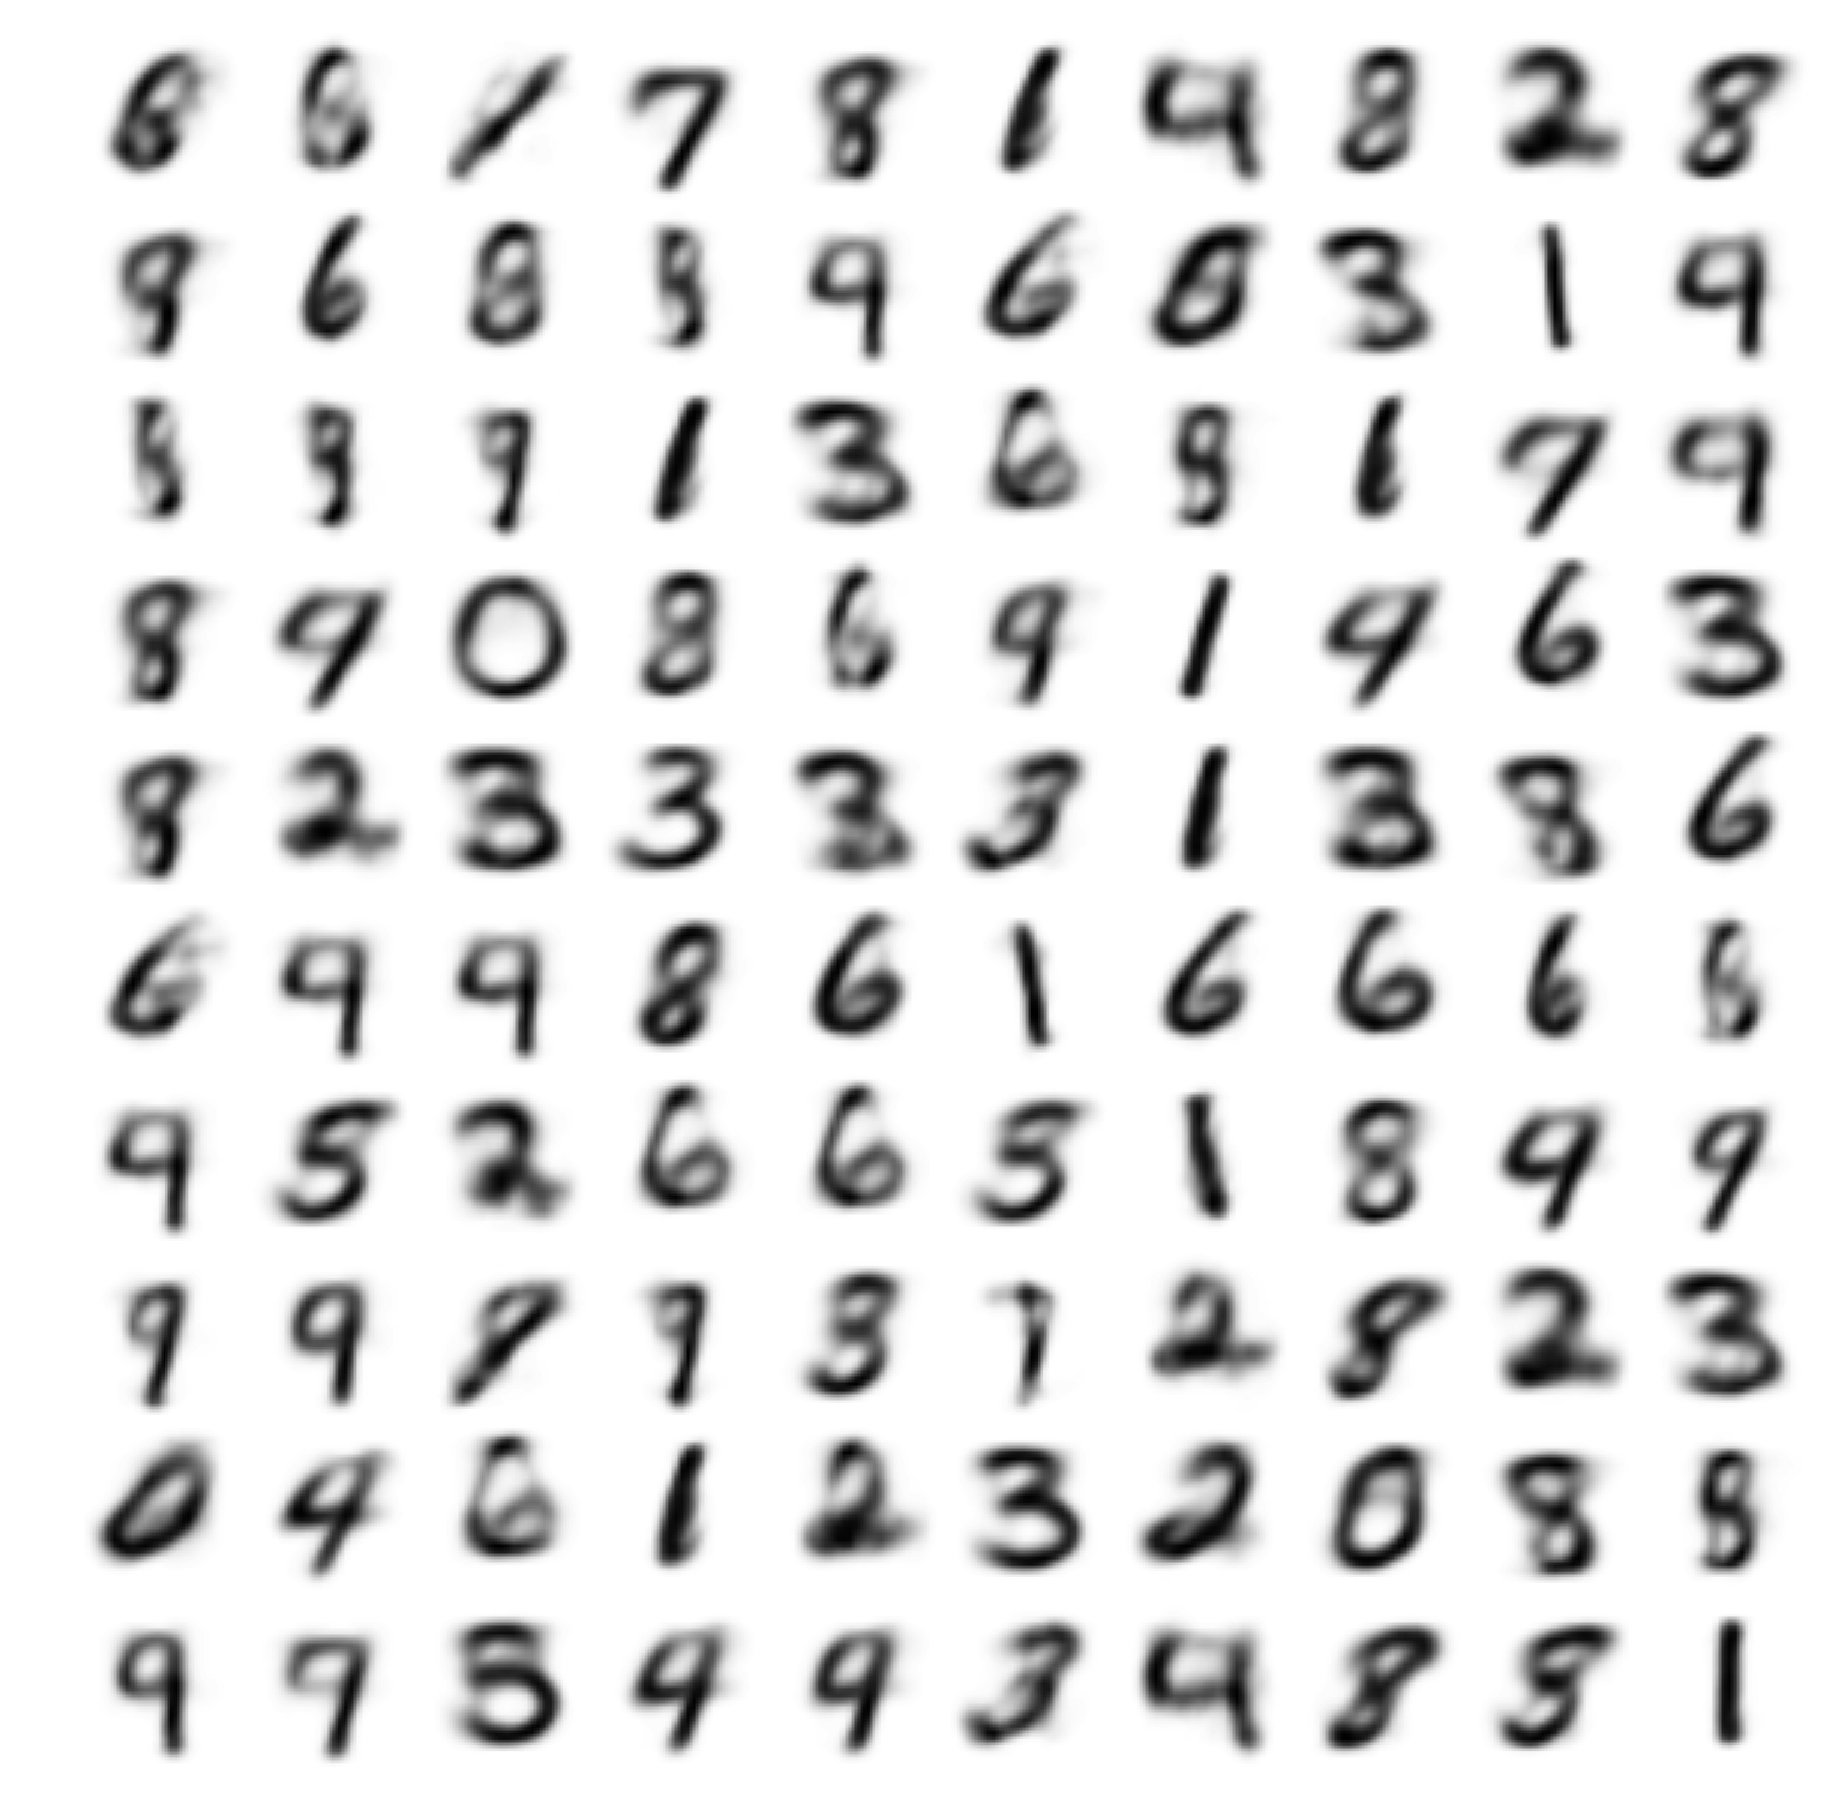
\includegraphics[width=0.23\textwidth]{assets/figures/mnist_100_sva_2-500.pdf}}
	\subfloat[五维潜在空间]{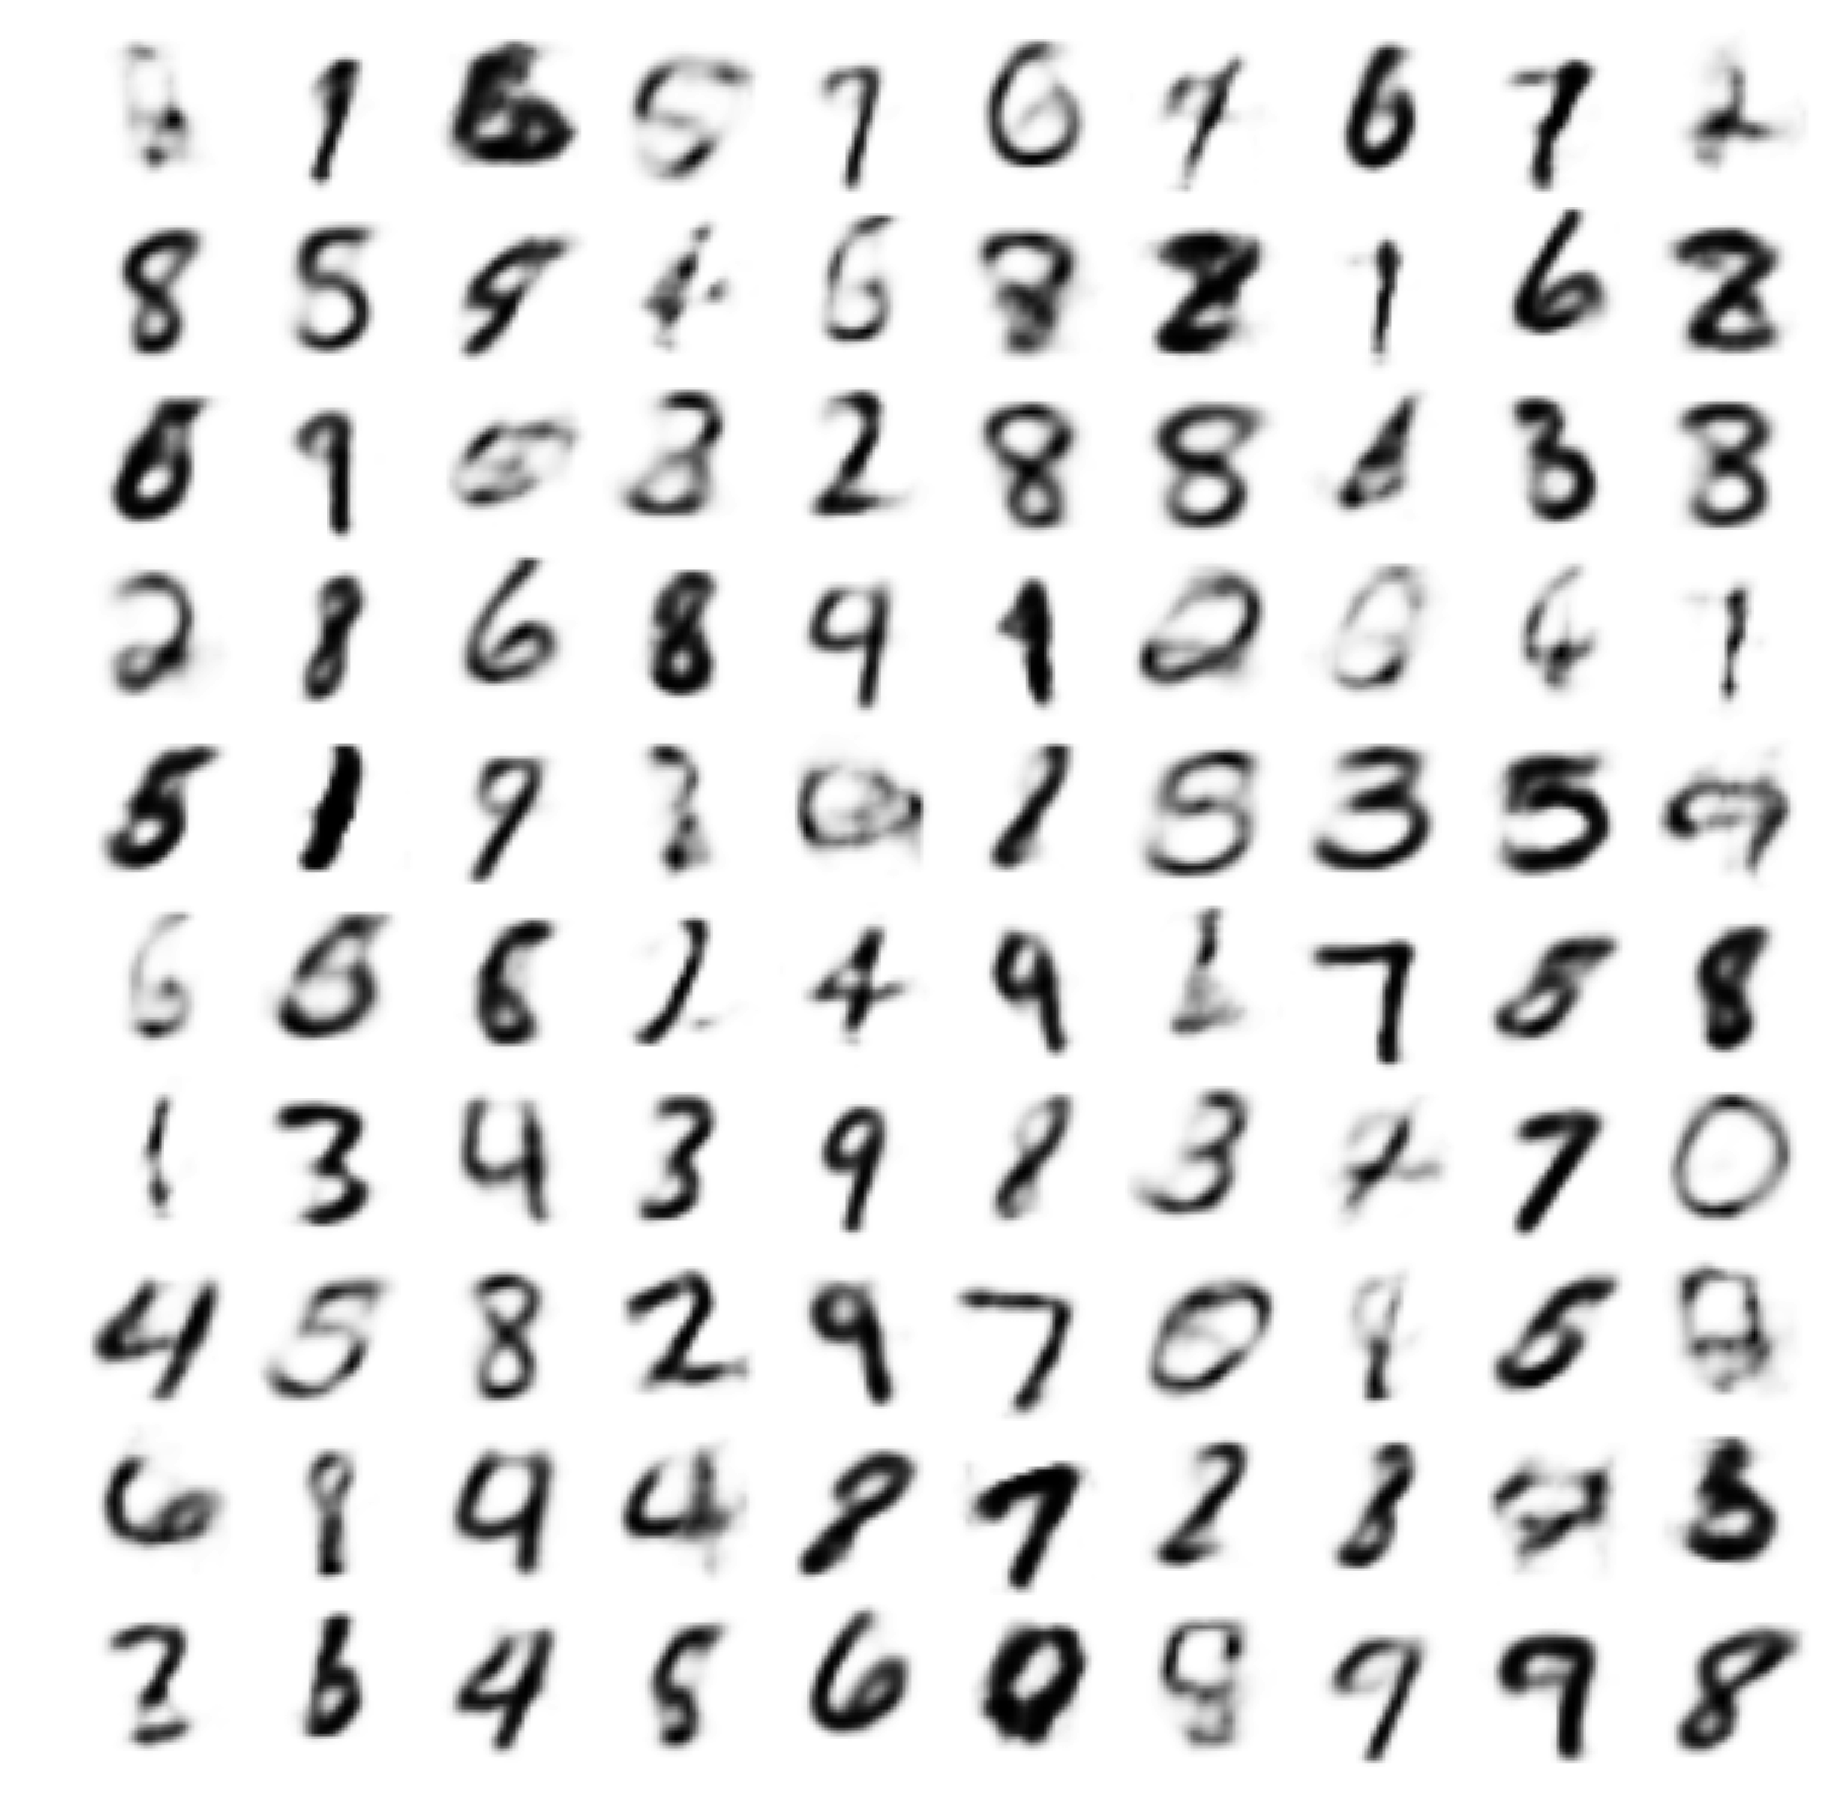
\includegraphics[width=0.23\textwidth]{assets/figures/mnist_100_sva_5-500.pdf}}
	\subfloat[十维潜在空间]{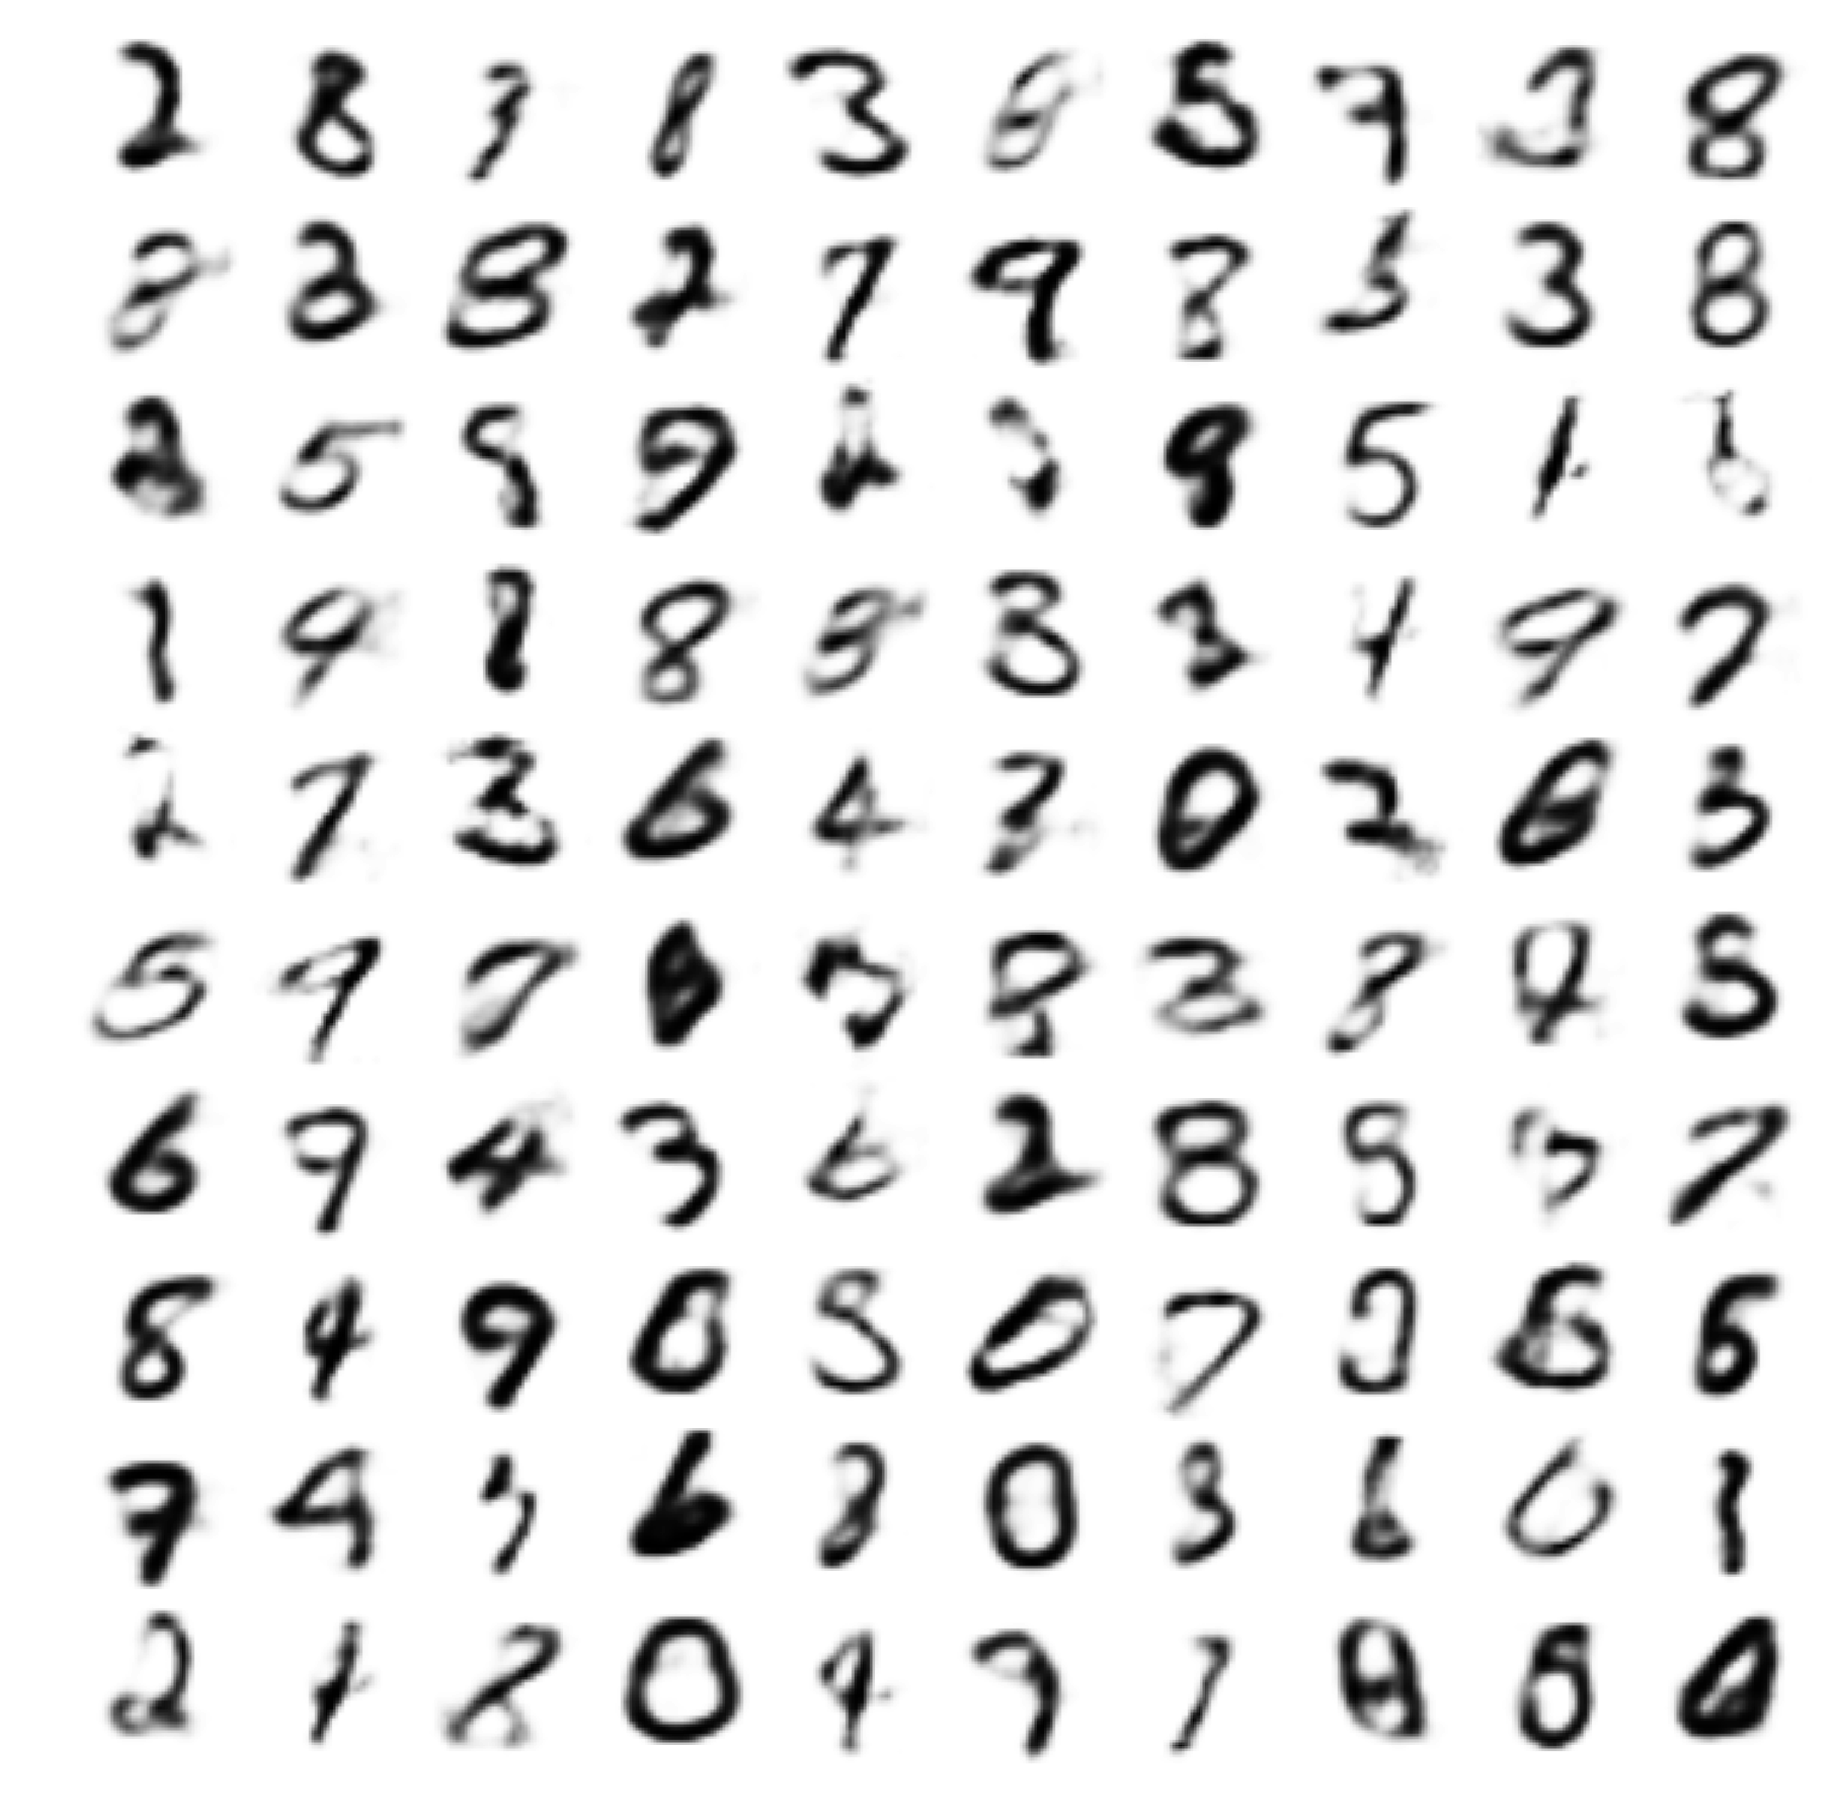
\includegraphics[width=0.23\textwidth]{assets/figures/mnist_100_sva_10-500.pdf}}
	\subfloat[二十维潜在空间]{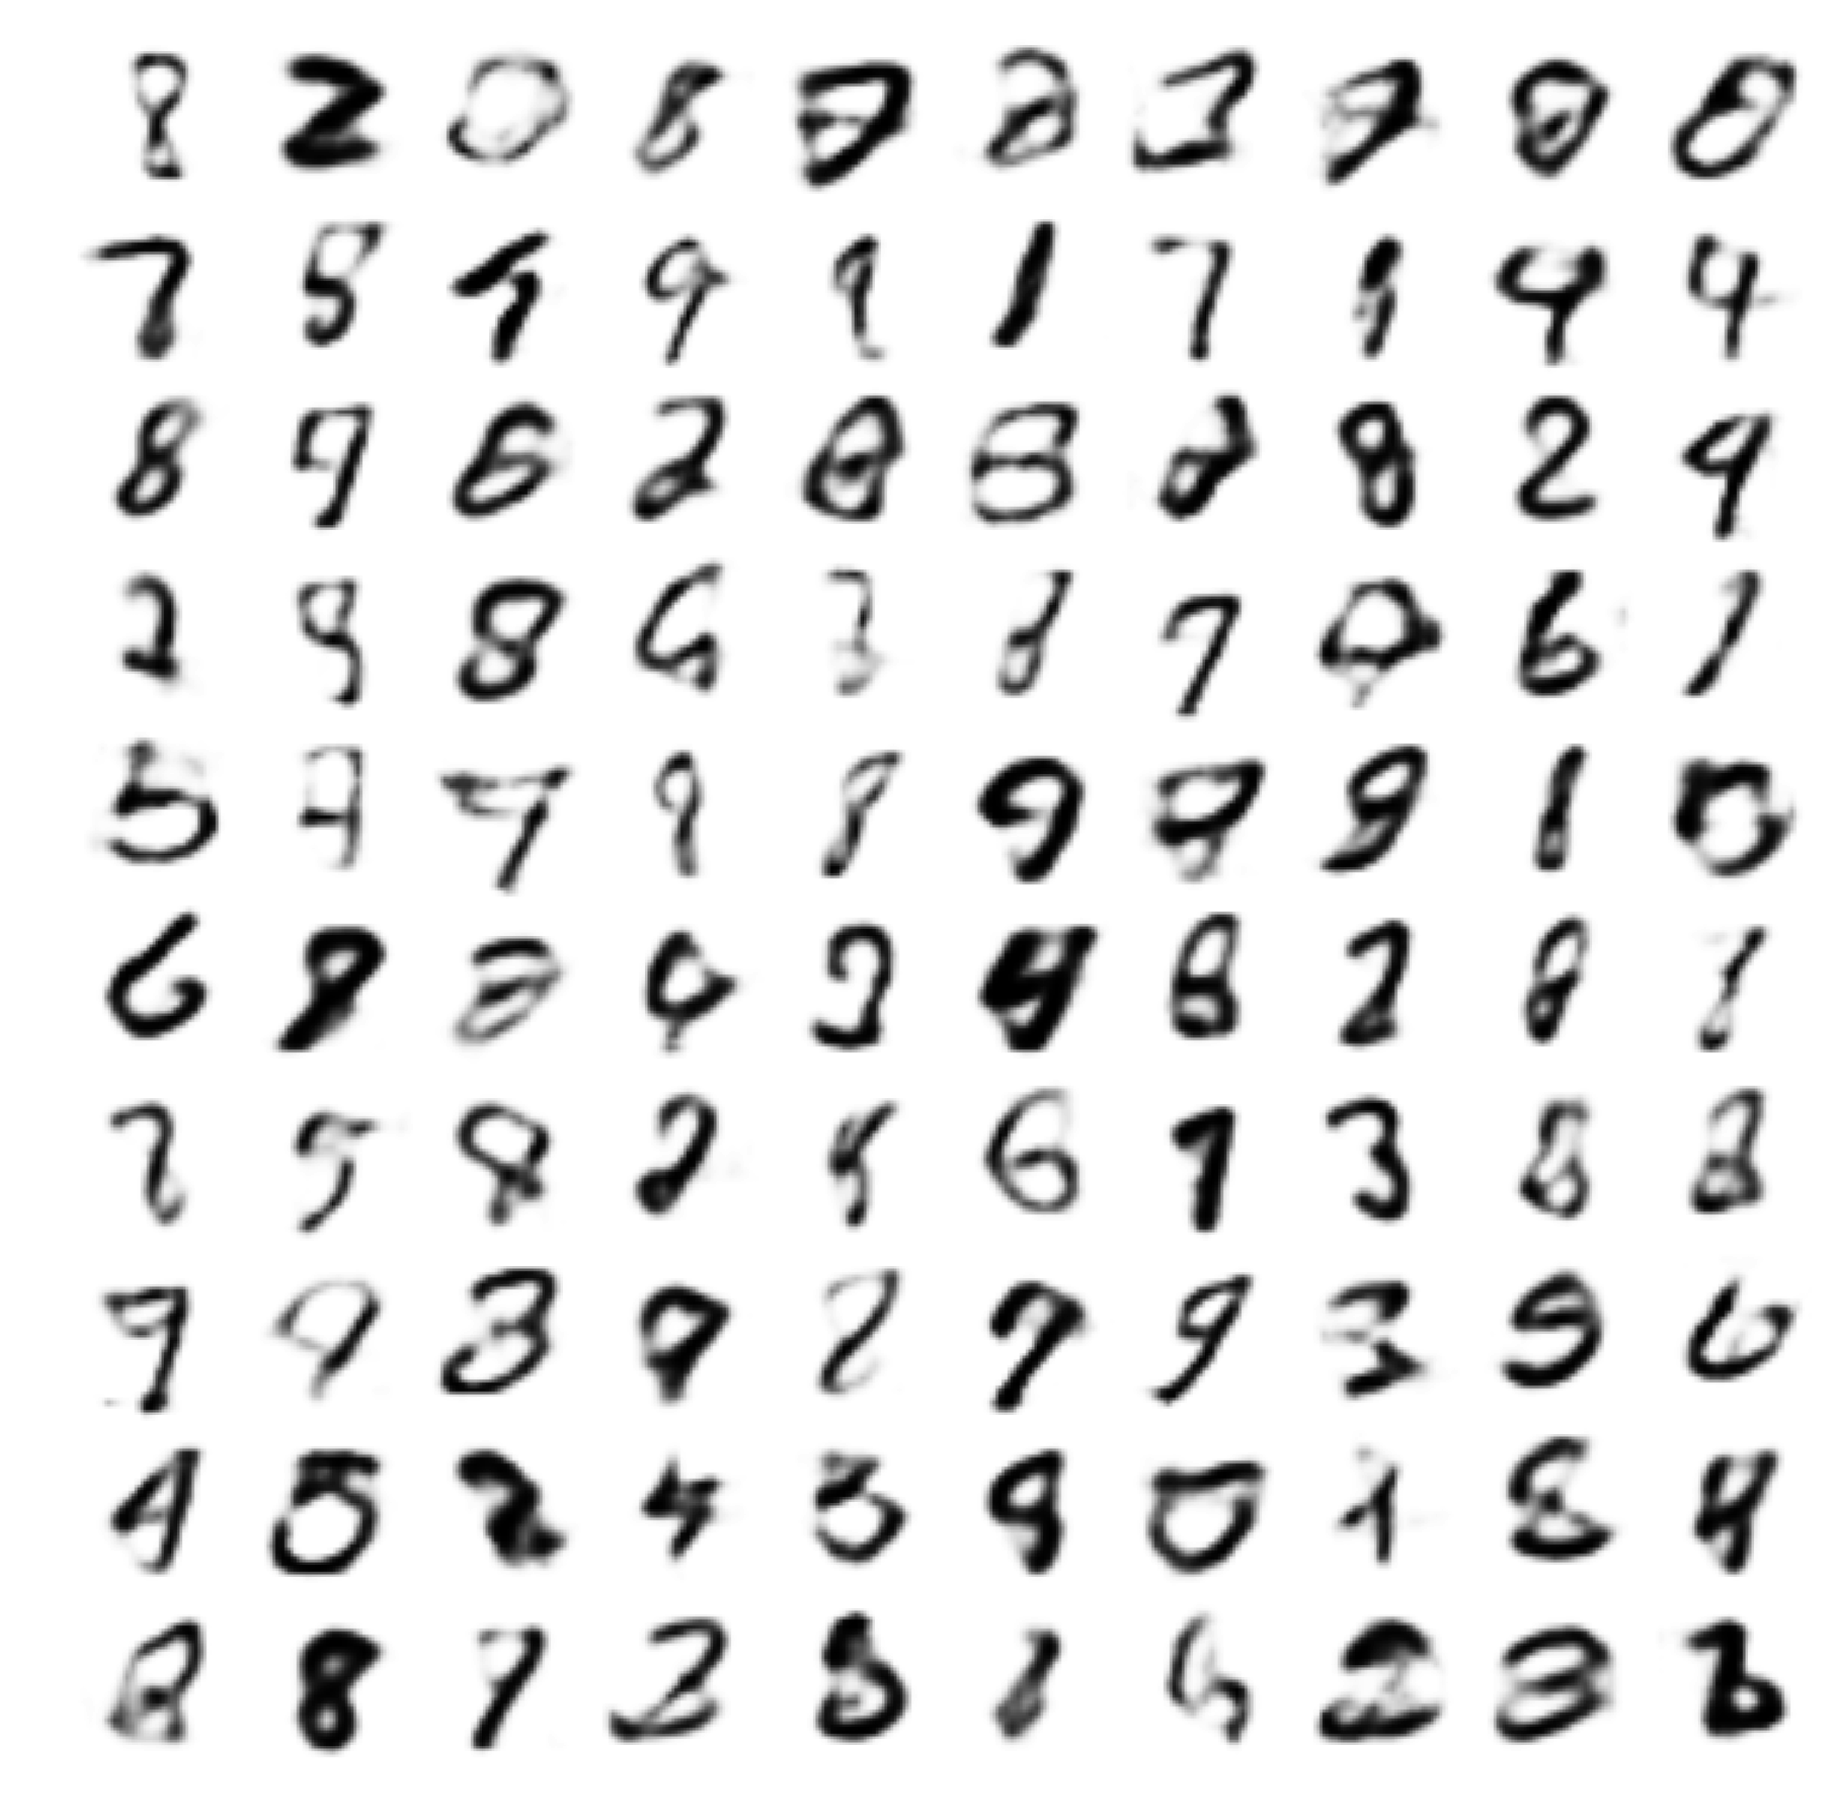
\includegraphics[width=0.23\textwidth]{assets/figures/mnist_100_sva_20-500.pdf}}
\caption{从不同潜在空间维数的 MNIST 生成模型中随机采样得到的图像。}
\label{fig:mnistsamples}
\end{figure}
